% !TEX root = knottedMain.tex
\documentclass[varwidth=\maxdimen]{standalone}

\usepackage{mathtools,amssymb,mathrsfs,dutchcal,upgreek,faktor,accents,etoolbox,multicol}
\usepackage[dvipsnames]{xcolor}
\definecolor{mygreen}{RGB}{	8,156,79 }
\usepackage{tikz,tikz-cd}
\usetikzlibrary{patterns,knots,arrows.meta,decorations.markings}
\tikzset{>={Straight Barb[scale=0.85]}}
\tikzcdset{
  cells={font=\everymath\expandafter{\the\everymath\displaystyle}},
  arrow style=tikz,
  diagrams={>={Straight Barb[scale=0.85]}},
  every label/.append style = {font = \small}
}


\begin{document}
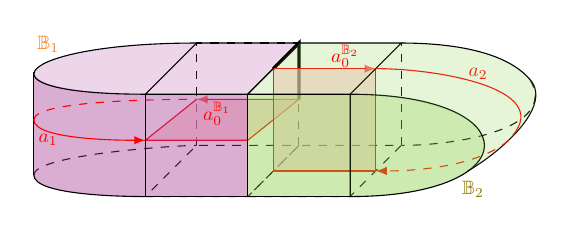
\begin{tikzpicture}[scale=1.3,every node/.style={scale=0.7}]
\clip (-1.9,-0.9) rectangle (3.1,0.9);

% B_1
    \draw[dashed]
        (-1.84,-0.54)  to[in=180,out=90,distance=0.2cm]
        (-0.25,-0.25);
    \fill[blue!45!red!80!white,fill opacity=0.4]
        (-0.75,0.25) to[out=180,in=-90,distance=0.2cm]
        (-1.84,0.47) --
         (-1.84,-0.54)  to[in=180,out=-90,distance=0.2cm]
         (-0.75,-0.75);
    \fill[blue!45!red!80!white,fill opacity=0.2,draw=black]
        (-0.25,0.75) to[out=180,in=180,distance=1.75cm] (-0.75,0.25);
    \draw
        (-1.84,-0.54) -- (-1.84,0.47);
    \draw
        (-1.84,-0.54)  to[in=180,out=-90,distance=0.2cm] (-0.75,-0.75);

    \draw[dashed,red]
        (-1.84,0)  to[in=180,out=90,distance=0.2cm] (-0.25,0.2);
    \draw[red,-latex]
        (-1.84,0)  to[in=180,out=-90,distance=0.2cm] (-0.75,-0.2);
    \draw[red] (-1.7,-0.2) node{$a_1$};
% ext region for B_1
    \draw[dashed]
        (-0.25,-0.25) rectangle (0.75,0.75);
    \draw[dashed]
        (-0.75,-0.75) -- (0.25,-0.75) -- 
        (0.75,-0.25) -- (-0.25,-0.25) -- (-0.75,-0.75);
    \fill[red!20,fill opacity=0.6,draw=red,-latex]
         (-0.25,0.2) -- (-0.75,-0.2) -- (0.25,-0.2) --
         (0.75,0.2) -- (-0.25,0.2);
    \fill[blue!45!red!80!white,fill opacity=0.2,draw=black]
        (-0.75,0.25) -- (0.25,0.25) -- 
        (0.75,0.75) -- (-0.25,0.75) -- (-0.75,0.25);

    \fill[blue!45!red!80!white,fill opacity=0.4,draw=black]
        (-0.75,-0.75) rectangle (0.25,0.25);

    \draw (-0.05,0.06) node[red]{$a_0^{\mathbb{B}_1}$};

    \draw[very thick] (0.75,0.2) -- (0.75,0.75) -- (0.5,0.5) ;
% B_2
    \draw 
        (2.4, -0.5) to[out=30,in=-50,distance=0.35cm] (3.01,0.39);

% ext region for B_2
    \draw[dashed]
        (1.75,-0.25) -- (1.75,0.75);
    \draw[dashed]
        (0.25,-0.75) -- (1.25,-0.75) -- 
        (1.75,-0.25) -- (0.75,-0.25) -- (0.25,-0.75);
    \fill[red!20,fill opacity=0.6,draw=red,-latex]
         (1.5,0.5) -- (1.5,-0.5) -- (0.5,-0.5) -- (0.5,0.5) --  (1.5,0.5);
    \fill[yellow!45!green!90!white,fill opacity=0.2,draw=black]
        (0.25,0.25) -- (1.25,0.25) -- 
        (1.75,0.75) -- (0.75,0.75) -- (0.25,0.25);

    \fill[yellow!45!green!90!white,fill opacity=0.4,draw=black]
        (0.25,-0.75) rectangle (1.25,0.25);
        
% front of B_2
    \draw[red,dashed,-latex]
        (2.8,-0.2)  to[out=-140,in=0,distance=0.4cm] (1.5,-0.5);
    \draw[red,]
        (1.5,0.5) to[out=0,in=50,distance=0.6cm] (2.84,-0.15) ;
    \draw[red] (2.5,0.45) node{$a_2$};
    
    \draw[dashed]
        (3.01,0.39)  to[out=-60,in=0,distance=0.55cm] (1.75,-0.25);
    \fill[yellow!45!green!90!white,fill opacity=0.4,draw=black]
        (1.25,0.25) to[out=0,in=0,distance=1.75cm] (1.25,-0.75) -- (1.25,0.25);
    \fill[yellow!45!green!90!white,fill opacity=0.2]
        (1.75,0.75) to[out=0,in=130,distance=0.4cm] 
        (3.01,0.39) to[in=30,out=-50,distance=0.35cm] 
        (2.4, -0.5) to[out=40,in=0,distance=0.72cm] 
        (1.25,0.25) -- (1.75,0.75) ;
    \draw
        (1.75,0.75) to[out=0,in=130,distance=0.4cm] 
        (3.01,0.39) ;


    \draw 
        (1.2,0.62) node[red]{$a_0^{\mathbb{B}_2}$}
        (2.45,-0.68) node[green!45!red]{$\mathbb{B}_2$}
        (-1.7,0.74) node[yellow!45!red]{$\mathbb{B}_1$};



\end{tikzpicture}


\end{document}